\chapter{Analiza sentimenta}
\label{ch:analiza-sentimenta}

Kaj pa kakšni novi podatki? Na primer z omrežja Twitter? V gradniku \widget{Corpus} kliknite na spustni meni in izberite \textit{election-2016-tweets.tab}. Ta korpus vsebuje 6000 tvitov Hillary Clinton in Donalda Trumpa v času predvolilne kampanje leta 2016.

Najprej moramo podatke predobdelati. Uporabili bomo poseben razčlenjevalnik enot (tokenizer) Tweet, ki je bil naučen na milijonih tvitov.\marginnote{Tviti pogosto zahtevajo posebno predprocesiranje. Najprej odstranite vse povezave (remove url), ker so te običajno nezanimive za analizo. Nato uporabite prednaučeni Tweet razčlenjevalnik, ki obdrži pojavnice kot so ‘@omemba’, ‘\#oznaka’ and emotikone :). Za konec uporabite še filter Regexp, ki odstrani ločila.}

Tokrat bomo imeli kar veliko unikatnih besed in stvari lahko postanejo precej počasne. Število besed lahko zmanjšamo tako, da uporabimo tehniko \textit{Document frequency}. Nižjo mejo bomo nastavili na 10, zgornjo pa na število dokumentov (6444) - tako bomo obdržali vse besede, ki se pojavijo v več kot 10 tvitih. Super, sedaj imamo znosnih 1000 enot.

Tokrat si bomo podatke pogledali z vidika čustev, ki jih tviti izražajo. Dodajte gradnik \widget{Sentiment Analysis}. Ta deluje tako, da besede iz dokumentov primerja s slovarjem pozitivnih in negativnih besed in na koncu izračuna oceno, kakšno čustvo zaznamuje tvit - pozitivno, negativno ali nevtralno.

Preden pa pogledamo rezultat, bomo morali še nekaj spremenljivk umakniti iz pogleda (glejte sliko). Uporabite gradnik \widget{Select Columns} in premaknite vse dodatne informacije o tvitih v polje \textit{meta attributes}.

\begin{figure}[h]
    \centering
    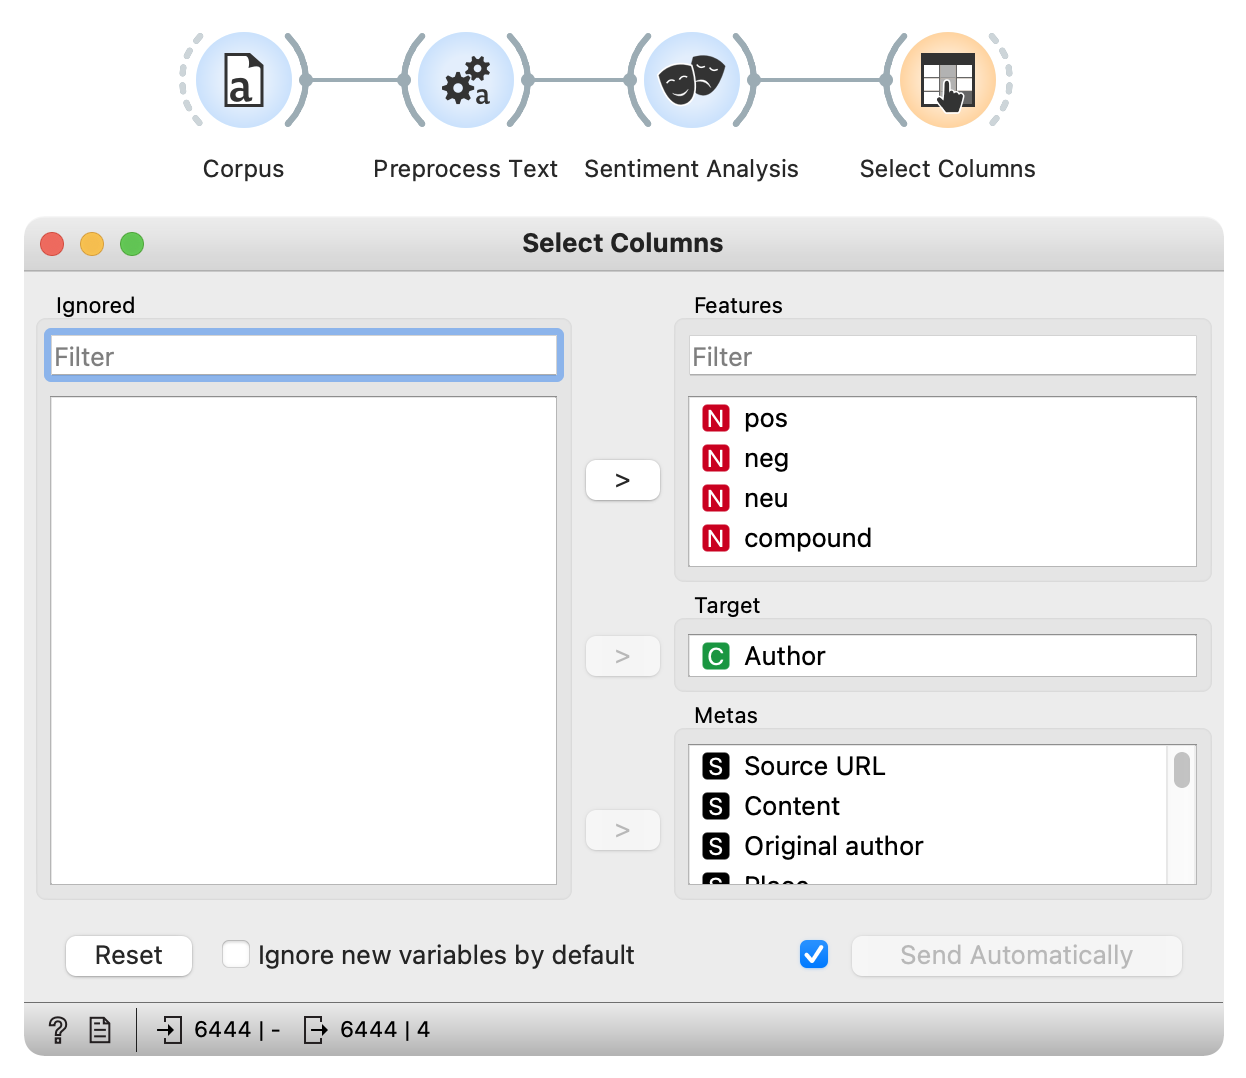
\includegraphics[width=\linewidth]{sentiment-1.png}%
    \caption{Nastavitve: 
    
    Razčlenjevalnik Tweet se uporablja za tvite, prednastavljeni razčlenjevalnik Regexp pa za običajno besedilo.
    
    Nastavite pogostost v dokumentih na 10. To bo odstranilo enote, ki se pojavijo v manj kot 10 tvitih.}
    \label{fig:011-sentiment}
\end{figure}
  
Nato dodajmo gradnik \widget{Heat Map}, ki prikazuje številske vrednosti stolpcev z barvno shemo. Modra polja imajo nizko vrednost, rumena pa visoko. Z drugimi besedami, kjer je vrednost spremenljivke \textit{compound} modra, je tvit negativen, kjer pa je rumena, je pozitiven.

\begin{figure*}[h]
    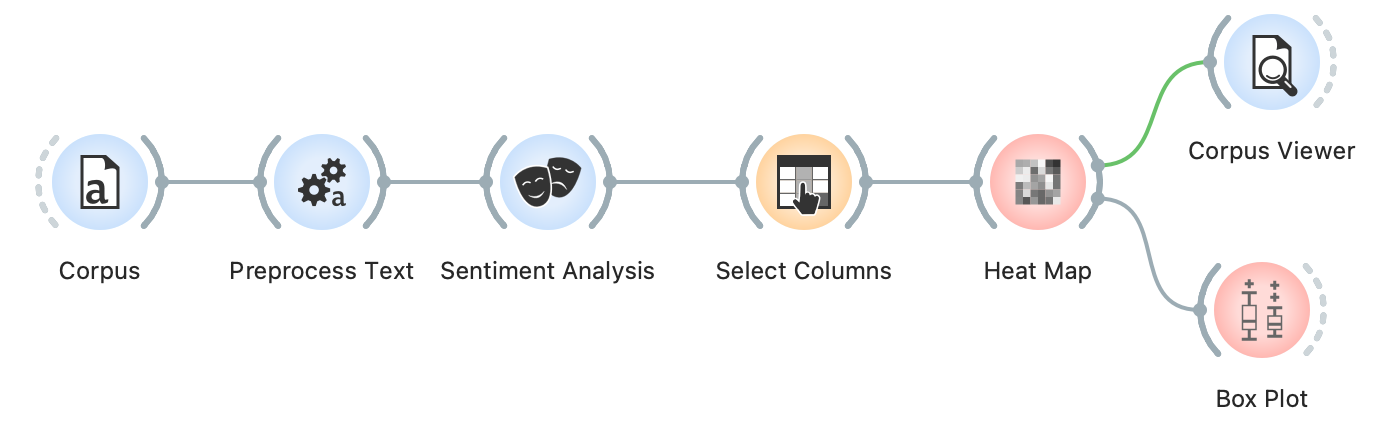
\includegraphics[width=\linewidth]{sentiment-workflow.png}%
    \caption{}
    \label{fig:011-sentiment-workflow}
\end{figure*}

V prikazu lahko označimo negativne tvite in jih pogledamo v \widget{Corpus Viewerju} ali pa pogledamo, kdo jih je napisal z gradnikom \widget{Box Plot}.

\begin{figure*}[h]
    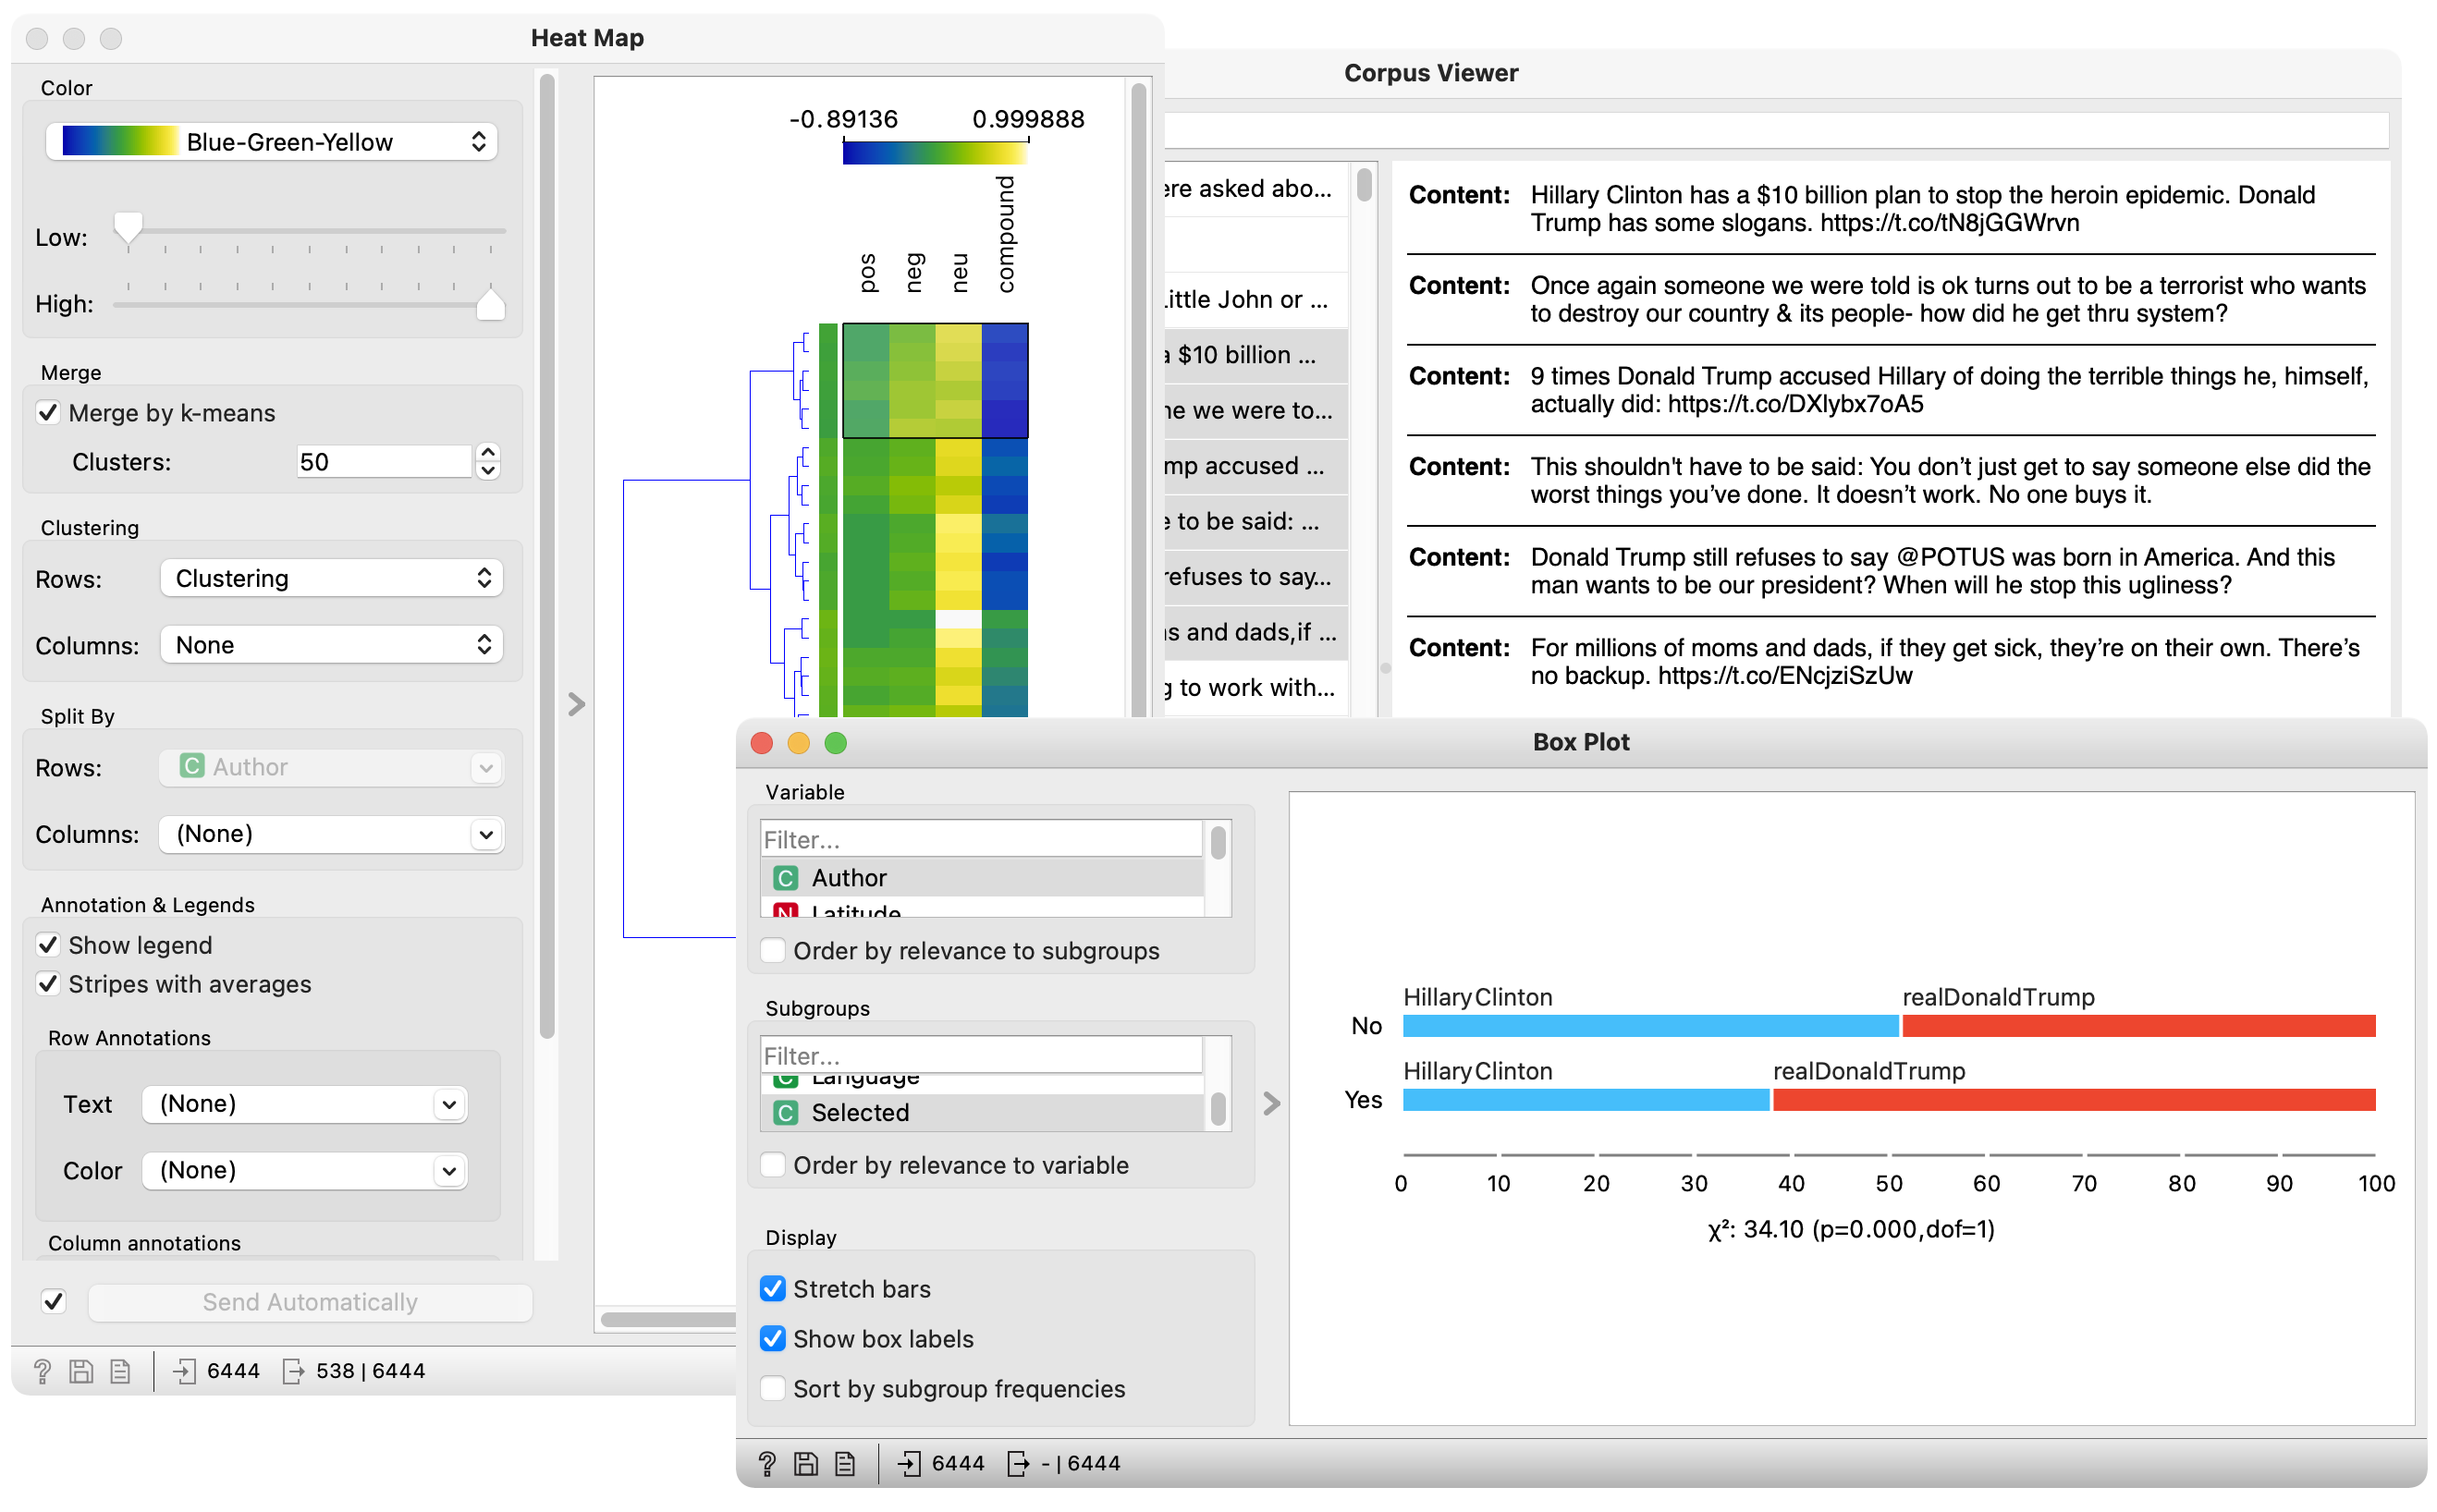
\includegraphics[width=\linewidth]{sentiment-2.png}%
    \caption{}
    \label{fig:011-sentiment2}
\end{figure*}